\section{The sequence column type}
\label{sec:appendix-sequence-type}

The type \texttt{bioseq.seq} stores a sequence together with the information
needed to interpret its symbols. A column declaration such as
\texttt{bioseq.seq('dna4',64)} specifies an alphabet and a packed storage-unit
width. The number 64 is neither a sequence-length limit nor the number of bits
used for each base. The examples assume that the extension has been installed
in the current database.

\subsection{Choose an alphabet and a packed width}

Choose the alphabet from the data that the column must preserve:
\begin{itemize}
  \item \texttt{dna4} represents A, C, G, and T. Use it when every input
    sequence consists of these four bases.
  \item \texttt{dna5} also represents N. Use it when an unknown base must keep
    its place in the sequence. This alphabet needs a build that registers it.
  \item A typed SQL input cast checks the symbols. Removing an unsupported
    symbol beforehand changes the sequence and moves every later position.
    It is a data transformation, not a harmless way to suppress an error.
\end{itemize}

This table is used throughout the first tutorial. Its primary key identifies
the record; its sequence column has an explicit alphabet.

\par\noindent\begin{minipage}{\linewidth}
\begin{lstlisting}[style=bioseq-appendix-sql]
CREATE TABLE resolved_reads (
    read_id bigint PRIMARY KEY,
    sequence bioseq.seq('dna4', 64) NOT NULL
) USING bioseq;

SET bioseq.index.insert_maintenance.enabled = on;
INSERT INTO resolved_reads VALUES
    (1, 'ACGTACGT'::bioseq.seq('dna4', 64)),
    (2, 'TTAA'::bioseq.seq('dna4', 64));
RESET bioseq.index.insert_maintenance.enabled;

SELECT read_id, sequence::text, bioseq.len(sequence)
FROM resolved_reads
ORDER BY read_id;
\end{lstlisting}
\end{minipage}

The output contains the same symbols that were inserted, with lengths 8 and
4. The maintenance setting permits enabled per-insert index work; it does not
select an alphabet or change the sequence type. Section~\ref{sec:appendix-configuration}
describes the index controls and their restrictions.

The accepted width arguments are 8, 16, 32, and 64 bits. A normal build
normalizes all four to 64-bit packed units. A build with all coordinate-width
variants enabled can retain the other widths. Therefore:
\begin{itemize}
  \item Treat the width as a request for a storage representation. Inspect the
    installed type modifier before comparing widths.
  \item Do not confuse packed units with bytes, bases, or SIMD lanes.
    Changing this argument does not by itself select a SIMD algorithm.
  \item Keep the default width unless measurements of the intended workload
    give a reason to change it.
\end{itemize}

\subsection{Inspect the stored modifier and name the measurement units}

The following probe distinguishes the requested widths from the modifiers
that PostgreSQL actually records. It deliberately puts the same 100-base
value in every column.

\par\noindent\begin{minipage}{\linewidth}
\begin{lstlisting}[style=bioseq-appendix-sql]
CREATE TABLE width_probe (
    id integer PRIMARY KEY,
    w8  bioseq.seq('dna4', 8),
    w16 bioseq.seq('dna4', 16),
    w32 bioseq.seq('dna4', 32),
    w64 bioseq.seq('dna4', 64)
) USING bioseq;

SELECT attname, format_type(atttypid, atttypmod) AS stored_type
FROM pg_attribute
WHERE attrelid = 'width_probe'::regclass
  AND attnum > 0 AND NOT attisdropped
ORDER BY attnum;
\end{lstlisting}
\end{minipage}

\par\noindent\begin{minipage}{\linewidth}
\begin{lstlisting}[style=bioseq-appendix-sql]
INSERT INTO width_probe VALUES (
    1,
    repeat('ACGT', 25)::bioseq.seq('dna4', 8),
    repeat('ACGT', 25)::bioseq.seq('dna4', 16),
    repeat('ACGT', 25)::bioseq.seq('dna4', 32),
    repeat('ACGT', 25)::bioseq.seq('dna4', 64)
);

SELECT bioseq.len(w8) AS symbols,
       bioseq.unit_len(w8) AS units_8,
       bioseq.unit_len(w16) AS units_16,
       bioseq.unit_len(w32) AS units_32,
       bioseq.unit_len(w64) AS units_64,
       w8::text = w64::text AS same_symbols
FROM width_probe;

DROP TABLE width_probe;
\end{lstlisting}
\end{minipage}

\texttt{bioseq.len} returns the number of symbols as a \texttt{bigint}.
\texttt{bioseq.unit\_len} returns the number of packed units needed for the
value's alphabet and width, also as a \texttt{bigint}. For DNA4, a 64-bit unit
holds 32 bases, so 100 bases need four units. In the normal build all four
unit counts above are four, and \texttt{same\_symbols} is true. These counts
do not include value headers, relation pages, or compression overhead; they
are not measurements of physical disk usage.

An empty sequence has zero symbols and zero packed units. It is different
from SQL \texttt{NULL}, which means that the value is missing.

\par\noindent\begin{minipage}{\linewidth}
\begin{lstlisting}[style=bioseq-appendix-sql]
SELECT bioseq.len(''::bioseq.seq('dna4', 64)) AS symbols,
       bioseq.unit_len(''::bioseq.seq('dna4', 64)) AS units,
       ''::bioseq.seq('dna4', 64) IS NULL AS is_missing;
-- symbols = 0; units = 0; is_missing = false
\end{lstlisting}
\end{minipage}

\subsection{Bind client inputs and convert widths}

Pass client sequence data as a text parameter and cast it explicitly at the
database boundary. This makes the intended alphabet visible and avoids
relying on how a client driver describes a parameter.

\par\noindent\begin{minipage}{\linewidth}
\begin{lstlisting}[style=bioseq-appendix-sql]
PREPARE insert_resolved_read(bigint, text) AS
INSERT INTO resolved_reads (read_id, sequence)
VALUES ($1, $2::bioseq.seq('dna4', 64));

EXECUTE insert_resolved_read(3, 'ACGTACGT');
DEALLOCATE insert_resolved_read;

SELECT ('ACGT'::bioseq.seq('dna4', 16)
               ::bioseq.seq('dna4', 64))::text;
-- ACGT
\end{lstlisting}
\end{minipage}

A cast between widths of the same alphabet preserves the symbols. It can be
a no-op when the build normalizes both widths. Where the widths differ, the
cast changes the requested representation; a lazy sequence need not be
copied into a new packed array immediately.

An alphabet is \emph{bound} when it is recorded in the sequence value.
Casting directly between two different bound alphabets is rejected, even
when the particular symbols would fit both alphabets. For example, a bound
DNA4 value cannot be cast directly to bound DNA5. Convert through text when
an alphabet change is intentional, and validate the destination contract.
The following optional example requires DNA5 support:

\par\noindent\begin{minipage}{\linewidth}
\begin{lstlisting}[style=bioseq-appendix-sql]
WITH candidates(sequence) AS (
    VALUES ('ACGT'::bioseq.seq('dna5', 64)),
           ('ACNT'::bioseq.seq('dna5', 64))
)
SELECT CASE WHEN sequence::text ~ '^[ACGT]*$'
            THEN sequence::text::bioseq.seq('dna4', 64)
       END AS resolved_sequence
FROM candidates;
\end{lstlisting}
\end{minipage}

The first result is ACGT; the second is \texttt{NULL}. The expression makes
the rejection policy explicit. If N is meaningful in the application, retain
DNA5 instead of changing its alphabet.

\subsection{Unbound values and client output}

A SQL expression can have the bare type \texttt{bioseq.seq}, without a type
modifier. This alone does not prove whether the value has a bound alphabet:
the value also carries this information. Current external-provider results
start as unbound ASCII sequences. Provider relation options do not turn
these results into a selected packed alphabet and width.

Length and text output are useful before binding. Alphabet-dependent
operations, such as returning a typed letter, creating a letter array, or
computing a reverse complement, need a bound alphabet. Bind and validate an
external value before using those operations. This example requests the
first 100 bases of the human mitochondrial reference from UCSC:

\par\noindent\begin{minipage}{\linewidth}
\begin{lstlisting}[style=bioseq-appendix-sql]
SELECT bioseq.len(sequence) AS bases, sequence::text
FROM bioseq_external.sequences
WHERE provider = 'ucsc'
  AND assembly_database = 'hg38'
  AND chromosome = 'chrM'
  AND start0 = 0 AND end0 = 100;
\end{lstlisting}
\end{minipage}

The provider example requires the external-provider installation and network
access. With DNA5 available, the expression below gives an explicit
validation boundary before the reverse complement. The text step is also
useful when changing an already bound alphabet; it is not required merely
to bind an unbound value.

\par\noindent\begin{minipage}{\linewidth}
\begin{lstlisting}[style=bioseq-appendix-sql]
SELECT bioseq.reverse_complement(
           sequence::text::bioseq.seq('dna5', 64))::text
FROM bioseq_external.sequences
WHERE provider = 'ucsc'
  AND assembly_database = 'hg38'
  AND chromosome = 'chrM'
  AND start0 = 0 AND end0 = 100;
\end{lstlisting}
\end{minipage}

Keep a sequence typed while the database searches or transforms it. Choose
the output form that the client actually needs:
\begin{itemize}
  \item Use \texttt{sequence::text} to return the complete string.
  \item Use \texttt{bioseq.to\_array(sequence)} only when the client needs a
    \texttt{bioseq.letter[]} array. Each element is a typed symbol.
  \item Use \texttt{sequence[:20]::text} or
    \texttt{sequence[-20:]::text} for a short prefix or suffix. Avoid
    returning a whole chromosome merely to display a preview.
\end{itemize}

\par\noindent\begin{minipage}{\linewidth}
\begin{lstlisting}[style=bioseq-appendix-sql]
SELECT read_id, sequence[:20]::text AS prefix,
       sequence[-20:]::text AS suffix,
       bioseq.to_array(sequence[:4]) AS first_four_letters
FROM resolved_reads
ORDER BY read_id;
\end{lstlisting}
\end{minipage}

\subsection{Compare values and use several sequence columns}

Sequence comparison uses the value's alphabet and logical symbols. Equal
symbols in the same alphabet compare equally across packed widths; physical
packing is not the meaning of equality. Alphabet identity participates in
comparison, so values bound to different alphabets should not be treated as
the same biological value merely because their text looks equal.

The explicit operator form also works when \texttt{bioseq} is absent from
\texttt{search\_path}:

\par\noindent\begin{minipage}{\linewidth}
\begin{lstlisting}[style=bioseq-appendix-sql]
SELECT 'ACGT'::bioseq.seq('dna4', 16)
       OPERATOR(bioseq.=)
       'ACGT'::bioseq.seq('dna4', 64) AS same_sequence;
-- true
\end{lstlisting}
\end{minipage}

A table may contain several sequence columns with different alphabets.
There is no table-wide rule that makes every sequence column DNA4. The
following optional schema requires DNA5 support:

\par\noindent\begin{minipage}{\linewidth}
\begin{lstlisting}[style=bioseq-appendix-sql]
CREATE TABLE paired_sequence_values (
    pair_id bigint PRIMARY KEY,
    resolved bioseq.seq('dna4', 64),
    with_unknowns bioseq.seq('dna5', 64)
) USING bioseq;

INSERT INTO paired_sequence_values VALUES (
    1, 'ACGT'::bioseq.seq('dna4', 64),
    'ACNT'::bioseq.seq('dna5', 64)
);

SELECT pair_id, bioseq.len(resolved), bioseq.len(with_unknowns)
FROM paired_sequence_values;

DROP TABLE paired_sequence_values;
\end{lstlisting}
\end{minipage}

This flexibility does not make mixed-alphabet searches interchangeable.
Choose compatible query and target alphabets explicitly. The separate
question of which search owns a result helper is covered in
Section~\ref{sec:appendix-joins}.

\subsection{Load sequences and inspect metadata work}

The file loader can fill a typed sequence column and map parsed header
fields to scalar columns. The following example assumes an accessible
FASTA file containing only A/C/G/T sequences, with UniProt-style headers
and one sequence destination column:

\par\noindent\begin{minipage}{\linewidth}
\begin{lstlisting}[style=bioseq-appendix-sql]
CREATE TABLE tutorial_loaded_reads (
    accession text NOT NULL,
    seq bioseq.seq('dna4', 64)
) USING bioseq;

SET bioseq.index.insert_maintenance.enabled = on;
SELECT bioseq.load(
    'tutorial_loaded_reads'::regclass,
    'landing_reads.fasta', 'uni_prot',
    ARRAY[('accession', 'accession')::bioseq.column_mapping]
);
RESET bioseq.index.insert_maintenance.enabled;

SELECT accession, bioseq.len(seq) AS bases, seq::text
FROM tutorial_loaded_reads
ORDER BY accession;

DROP TABLE tutorial_loaded_reads;
\end{lstlisting}
\end{minipage}

The path is read by the PostgreSQL server, not the SQL client. The result of
\texttt{bioseq.load} is the loaded-record count. The loader accepts one
bound sequence destination, rejects identity and generated columns, and
requires a default for an unmapped \texttt{NOT NULL} scalar column.

Typed SQL casts and bulk file input do not have identical validation rules.
The bulk reader has path-dependent, permissive handling of unsupported
bytes. Loading N-bearing input into DNA4 can shorten a sequence and shift
coordinates. Validate the input alphabet first when positions must be
preserved. Section~\ref{sec:app-local-ingestion} explains these restrictions,
gzip input, header formats, and the choice between index maintenance during
loading and an index update afterward.

The two statements below ask for different work. The first requests length
and an A count; the second also asks the server to produce the complete
sequence string.

\par\noindent\begin{minipage}{\linewidth}
\begin{lstlisting}[style=bioseq-appendix-sql]
EXPLAIN (ANALYZE, VERBOSE, COSTS OFF)
SELECT bioseq.len(sequence), bioseq.symbol_count(sequence, 'A')
FROM resolved_reads;

EXPLAIN (ANALYZE, VERBOSE, COSTS OFF)
SELECT bioseq.len(sequence), sequence::text
FROM resolved_reads;
\end{lstlisting}
\end{minipage}

On an eligible \texttt{BioseqScan}, \texttt{Bioseq Fetched From Meta}
identifies metadata projections, while \texttt{Bioseq Projected Columns}
lists the supplied columns. A metadata shortcut for one expression does
not remove the payload read required by another expression in the same
query. Inspect the application's complete query.

\subsection{Diagnose input errors and check the schema}

\begin{center}
\small
\begin{tabular}{@{}lp{0.72\linewidth}@{}}
\toprule
SQLSTATE & Meaning in these examples \\
\midrule
\texttt{22P02} & A typed input contains a symbol absent from its alphabet;
  for example, \texttt{'ACGN'::bioseq.seq('dna4',64)}. \\
\texttt{42804} & A cast or assignment tries to change an already bound
  alphabet, or an operation requires an alphabet that is not bound. \\
\texttt{22023} & An unsupported alphabet name or width is used in a type
  modifier. A missing DNA5 build fails here before a DNA4-to-DNA5 cast can
  reach the alphabet-compatibility check. \\
\texttt{42883} & PostgreSQL cannot resolve the requested operator or
  signature; an absent \texttt{bioseq} schema in the search path is one
  possible cause. \\
\bottomrule
\end{tabular}
\end{center}

Check these points before choosing a production schema:
\begin{itemize}
  \item Does the data include N, and does the installed build provide the
    required alphabet?
  \item Which packed width does \texttt{format\_type} actually report?
  \item Do missing values and empty sequences have different meanings in
    the application?
  \item Will insertion maintain the required indexes, or will a later
    explicit update prepare them for search?
  \item Do query and target columns have compatible alphabets?
  \item Which queries need full strings, and which need only lengths,
    counts, or slices?
\end{itemize}

Keep error reports small: record the failing input's identifier, alphabet,
and length instead of printing an entire large sequence. The first tutorial
is now complete; its demonstration table can be removed.

\par\noindent\begin{minipage}{\linewidth}
\begin{lstlisting}[style=bioseq-appendix-sql]
DROP TABLE resolved_reads;
\end{lstlisting}
\end{minipage}

\section{Slices, concatenation, and sequence transforms}
\label{sec:appendix-sequence-transforms}

Sequence operations use zero-based positions and half-open intervals.
They return typed values, so a slice can remain a sequence while it is
reversed, joined to another piece, or searched. Converting the result to
text is a separate request for its symbols.

\subsection{Create a small table and read positions}

\par\noindent\begin{minipage}{\linewidth}
\begin{lstlisting}[style=bioseq-appendix-sql]
CREATE TABLE slice_reads (
    read_id integer PRIMARY KEY,
    sequence bioseq.seq('dna4', 64) NOT NULL
) USING bioseq;

SET bioseq.index.insert_maintenance.enabled = on;
INSERT INTO slice_reads VALUES
    (1, 'ACGTA'::bioseq.seq('dna4', 64)),
    (2, 'TTCCA'::bioseq.seq('dna4', 64)),
    (3, 'GGACT'::bioseq.seq('dna4', 64));
RESET bioseq.index.insert_maintenance.enabled;
\end{lstlisting}
\end{minipage}

\begin{figure}[htbp]
\centering
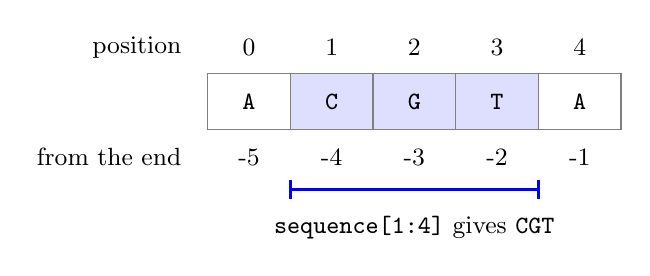
\begin{tikzpicture}[x=1.05cm,y=0.72cm,font=\small]
  \foreach \x/\base/\neg in {0/A/-5,1/C/-4,2/G/-3,3/T/-2,4/A/-1} {
    \ifnum\x>0\ifnum\x<4
      \fill[blue!13] (\x,0) rectangle +(1,1);
    \fi\fi
    \draw[gray] (\x,0) rectangle +(1,1);
    \node at (\x+0.5,0.5) {\texttt{\base}};
    \node at (\x+0.5,1.45) {\x};
    \node at (\x+0.5,-0.48) {\neg};
  }
  \node[anchor=east] at (-0.2,1.45) {position};
  \node[anchor=east] at (-0.2,-0.48) {from the end};
  \draw[very thick,blue] (1,-1.05) -- (4,-1.05);
  \draw[very thick,blue] (1,-0.88) -- (1,-1.22);
  \draw[very thick,blue] (4,-0.88) -- (4,-1.22);
  \node[anchor=north] at (2.5,-1.35)
    {\texttt{sequence[1:4]} gives \texttt{CGT}};
\end{tikzpicture}
\caption{The slice includes positions 1, 2, and 3. Position 4 is the
excluded end. Negative indexes count backward from the sequence end.}
\label{fig:appendix-slice-positions}
\end{figure}

An index returns one \texttt{bioseq.letter}; a slice returns
\texttt{bioseq.seq}. For a sequence of length $n$:
\begin{itemize}
  \item Index 0 is the first symbol; index $n-1$ is the last.
  \item Index $-1$ is the last symbol; index $-n$ is the first.
  \item An index outside the sequence returns \texttt{NULL}.
  \item A slice \texttt{[start:end]} includes \texttt{start} and excludes
    \texttt{end}. Omitting the start means 0; omitting the end means $n$.
\end{itemize}

\subsection{Normalize bounds and distinguish empty values from NULL}

A negative bound is counted from the end, then a slice bound is clamped to
the interval $[0,n]$. If the normalized end is at or before the normalized
start, the result is an empty sequence. No symbol is read outside the value.
The following expressions form a compact operation table for ACGTA:

\par\noindent\begin{minipage}{\linewidth}
\begin{lstlisting}[style=bioseq-appendix-sql]
SELECT sequence[0]::text AS first,
       sequence[-1]::text AS last,
       sequence[5] IS NULL AS past_end,
       sequence[1:4]::text AS middle,
       sequence[:2]::text AS prefix,
       sequence[2:]::text AS suffix,
       sequence[1:-1]::text AS inner_bases,
       sequence[-4:-1]::text AS same_inner_bases,
       sequence[:-2]::text AS without_last_two,
       sequence[-3:]::text AS last_three,
       sequence[-100:100]::text AS clamped,
       bioseq.len(sequence[3:3]) AS empty_length,
       sequence[4:2] IS NULL AS empty_is_missing
FROM slice_reads WHERE read_id = 1;
\end{lstlisting}
\end{minipage}

The results are A, A, true, CGT, AC, GTA, CGT, CGT, ACG, GTA, ACGTA, 0,
and false. Splitting at position 2 gives \texttt{AC} and \texttt{GTA}; joining
those pieces reconstructs ACGTA without repeating a boundary symbol.

An omitted bound and a bound whose value is SQL \texttt{NULL} differ.
\texttt{sequence[:2]} returns a prefix, whereas
\texttt{sequence[NULL::bigint:2]} returns \texttt{NULL}. A NULL sequence
also produces NULL when indexed or sliced. If a client uses NULL to mean
``use the start of the sequence'', express that policy explicitly:

\par\noindent\begin{minipage}{\linewidth}
\begin{lstlisting}[style=bioseq-appendix-sql]
PREPARE optional_slice_start(bigint) AS
SELECT CASE WHEN $1 IS NULL THEN sequence[:2]
            ELSE sequence[$1:2]
       END AS selected_sequence
FROM slice_reads WHERE read_id = 1;

EXECUTE optional_slice_start(NULL); -- AC
EXECUTE optional_slice_start(1);    -- C
DEALLOCATE optional_slice_start;
\end{lstlisting}
\end{minipage}

Sequence subscripting is read-only and one-dimensional, with a step of one.
It does not provide a Python-style step argument or multidimensional array
access. To return every second symbol as separate rows, generate the desired
positions explicitly:

\par\noindent\begin{minipage}{\linewidth}
\begin{lstlisting}[style=bioseq-appendix-sql]
SELECT r.read_id, p.position, r.sequence[p.position]::text
FROM slice_reads AS r
CROSS JOIN LATERAL
    generate_series(0::bigint, bioseq.len(r.sequence) - 1, 2)
    AS p(position)
WHERE r.read_id = 1
ORDER BY p.position;
-- positions 0, 2, 4 contain A, G, A
\end{lstlisting}
\end{minipage}

\subsection{Concatenate sequences, text, and arrays}

The BioSeqDB concatenation operator accepts compatible sequences and can
also combine a sequence with text, \texttt{text[]}, or
\texttt{bioseq.letter[]}, on either side. Use ordinary \texttt{||} when
the operator is visible through \texttt{search\_path}, or use the explicit
\texttt{OPERATOR(bioseq.||)} spelling below.

\par\noindent\begin{minipage}{\linewidth}
\begin{lstlisting}[style=bioseq-appendix-sql]
SELECT (sequence[:2] OPERATOR(bioseq.||) sequence[2:])::text
           AS reconstructed,
       (sequence[:3] OPERATOR(bioseq.||) 'TA'::text)::text
           AS append_text,
       ('AC'::text OPERATOR(bioseq.||) sequence[2:])::text
           AS prepend_text,
       (sequence[:2] OPERATOR(bioseq.||)
           ARRAY['G', 'TA']::text[])::text AS append_text_array,
       (ARRAY['AC']::text[] OPERATOR(bioseq.||)
           sequence[2:])::text AS prepend_text_array,
       (sequence[:2] OPERATOR(bioseq.||)
           bioseq.to_array(sequence[2:]))::text AS append_letters,
       (bioseq.to_array(sequence[:2]) OPERATOR(bioseq.||)
           sequence[2:])::text AS prepend_letters
FROM slice_reads WHERE read_id = 1;
-- Each result is ACGTA.
\end{lstlisting}
\end{minipage}

The array forms join their elements in order. A text-array element can
contain more than one symbol. Letter-array elements must have one consistent
alphabet, compatible with the bound sequence. Both array forms accept an
empty array as an identity and reject NULL elements and multidimensional
arrays.

The alphabet rules apply to the whole operation:
\begin{itemize}
  \item Two bound sequences must have the same alphabet. Different packed
    widths do not implicitly change that alphabet.
  \item Text is validated when it adopts the bound sequence's alphabet.
    Appending \texttt{'N'} to DNA4 therefore fails with SQLSTATE
    \texttt{22P02}; it does not silently produce DNA5.
  \item A nonempty letter array cannot supply the missing alphabet of an
    unbound sequence. Bind the sequence first.
  \item A NULL operand gives a NULL result. Empty text, an empty array, and
    an empty typed sequence are valid values, not missing operands.
\end{itemize}

Use \texttt{COALESCE} only when the application intentionally interprets a
missing value as an empty sequence:

\par\noindent\begin{minipage}{\linewidth}
\begin{lstlisting}[style=bioseq-appendix-sql]
SELECT (sequence OPERATOR(bioseq.||)
           COALESCE(NULL::bioseq.seq('dna4', 64),
                    ''::bioseq.seq('dna4', 64)))::text
FROM slice_reads WHERE read_id = 1;
-- ACGTA
\end{lstlisting}
\end{minipage}

\subsection{Reverse a sequence or take its reverse complement}

Reversal changes symbol order. A reverse complement also replaces each
symbol by its complement in the bound alphabet. The following example makes
the distinction visible:

\par\noindent\begin{minipage}{\linewidth}
\begin{lstlisting}[style=bioseq-appendix-sql]
SELECT sequence::text AS original,
       bioseq.reverse(sequence)::text AS reversed,
       bioseq.reverse_complement(sequence)::text AS reverse_complement,
       bioseq.reverse(sequence[1:4])::text AS reversed_middle
FROM slice_reads WHERE read_id = 1;
-- ACGTA | ATGCA | TACGT | TGC
\end{lstlisting}
\end{minipage}

An empty input remains empty; a NULL input remains NULL. Reversal itself
does not require a complement rule. Reverse complement requires a bound
alphabet with a complete complement mapping. An unbound input fails with
SQLSTATE \texttt{42804}; an alphabet without a complete mapping is not a
supported reverse-complement input. Bind external values as described in
Section~\ref{sec:appendix-sequence-type}.

For strand-aware output, make the policy for an unknown strand visible.
This example uses 1 for forward and $-1$ for reverse, and returns NULL for
any other value:

\par\noindent\begin{minipage}{\linewidth}
\begin{lstlisting}[style=bioseq-appendix-sql]
WITH strands(read_id, strand) AS (
    VALUES (1, 1), (2, -1), (3, 0)
)
SELECT r.read_id,
       (CASE s.strand
          WHEN 1 THEN r.sequence
          WHEN -1 THEN bioseq.reverse_complement(r.sequence)
          ELSE NULL::bioseq.seq('dna4', 64)
        END)::text AS oriented_sequence
FROM slice_reads AS r
JOIN strands AS s USING (read_id)
ORDER BY r.read_id;
\end{lstlisting}
\end{minipage}

\subsection{Measure and build a derived sequence}

Measure the expression that the next operation will consume.
\texttt{bioseq.len} counts its symbols; \texttt{bioseq.unit\_len} counts
its packed units, rather than bytes copied during evaluation.

\par\noindent\begin{minipage}{\linewidth}
\begin{lstlisting}[style=bioseq-appendix-sql]
SELECT bioseq.len(sequence) AS source_symbols,
       bioseq.unit_len(sequence) AS source_packed_units,
       bioseq.len(bioseq.reverse(sequence[1:-1])
           OPERATOR(bioseq.||) 'AC'::text) AS derived_symbols
FROM slice_reads WHERE read_id = 1;
-- 5 source symbols; 5 derived symbols
\end{lstlisting}
\end{minipage}

A derived target can be assembled without first converting the source to
text. Here the query removes one base from each end, reverses the remaining
piece, and attaches a prefix and suffix. The intermediate expression stays
typed; only the displayed result is text.

\par\noindent\begin{minipage}{\linewidth}
\begin{lstlisting}[style=bioseq-appendix-sql]
WITH derived AS (
    SELECT read_id,
           'AC'::text OPERATOR(bioseq.||)
             bioseq.reverse(sequence[1:-1])
             OPERATOR(bioseq.||) 'GT'::text AS target
    FROM slice_reads
)
SELECT read_id, bioseq.len(target), target::text
FROM derived
ORDER BY read_id;
-- For read 1: 7 symbols, ACTGCGT.
\end{lstlisting}
\end{minipage}

\subsection{Search a derived region}

A slice can be the target argument of \texttt{mmsearch}. The following
statement illustrates the SQL form on the small fixture:

\par\noindent\begin{minipage}{\linewidth}
\begin{lstlisting}[style=bioseq-appendix-sql]
SELECT read_id, sequence[1:-1]::text AS searched_region
FROM slice_reads
WHERE public.mmsearch(sequence[1:-1],
               'CGT'::bioseq.seq('dna4', 64));
\end{lstlisting}
\end{minipage}

This three-base query is a syntax example, not a claim that the default
seeding and chaining thresholds will report a match. The search tutorial
uses inputs long enough for the configured algorithm. When a transformed
target is evaluated, its original persisted minimizer index does not
describe that logical sequence; the current transformed-target path
recomputes the required minimizers. Search coordinates refer to the derived
value. For a plain slice, let $a$ be its start after resolving negative bounds
and clamping to the source length. Adding $a$ converts its target positions
back to the source. Reversal and concatenation require
their own coordinate mapping.

If projecting search helpers, pass the exact target expression, such as
\nolinkurl{bioseq.target_start(sequence[1:-1])}. A base-column or row-key
argument is only sufficient when it identifies one search unambiguously.
Separate search owners and SQL query levels matter when several searches
refer to the same source; adding aliases alone does not make every stacked
predicate supported. Section~\ref{sec:appendix-joins} gives supported join and
self-join patterns.

\subsection{See when the symbols are produced}

A slice can initially describe a range of its source. Materialization means
producing the symbols required by a later consumer. Asking only for a
slice's length is different from asking for its complete string:

\par\noindent\begin{minipage}{\linewidth}
\begin{lstlisting}[style=bioseq-appendix-sql]
EXPLAIN (ANALYZE, VERBOSE, COSTS OFF)
SELECT bioseq.len(sequence[1:-1])
FROM slice_reads;

EXPLAIN (ANALYZE, VERBOSE, COSTS OFF)
SELECT sequence[1:-1]::text
FROM slice_reads;
\end{lstlisting}
\end{minipage}

Depending on the plan and output format, the slice explanation includes:
\begin{itemize}
  \item \texttt{Projection Mode}, \texttt{Source Pieces}, and
    \texttt{Estimated Piece Boundaries}: how the projection refers to source
    pieces and how many piece boundaries are estimated.
  \item \texttt{Slice Recipe}: each operation, its expression, dependencies,
    and slice bounds. The recipe describes how the value is assembled.
  \item \texttt{Slice Materialization}: the expression that needs symbols,
    the mechanism and reason, its dependencies, encoding, and cache scope.
  \item With costs enabled, estimated symbols and bytes. The current byte
    estimate is one byte per symbol, not a packed-storage forecast. With
    \texttt{ANALYZE}, measured calls, input and output symbols,
    \texttt{Actual Bytes}, reused calls, and peak retained bytes. Timing
    fields depend on timing being enabled.
\end{itemize}

Section~\ref{sec:appendix-explain} describes the complete plan format.
Estimated work is not measured work, and a stored recipe does not promise
that every later consumer avoids copying. A text result or letter array
still needs symbols. Inspect the actual query and its plan before removing
an operation merely because it appears to cause materialization.

\subsection{Common mistakes and cleanup}

Check the smallest expression that fails:
\begin{itemize}
  \item Unexpected NULL slice: distinguish an omitted bound from an
    explicitly NULL bound, and check the input value itself.
  \item Unresolved concatenation: use \texttt{OPERATOR(bioseq.||)} or
    make the schema visible through \texttt{search\_path}.
  \item Invalid text or incompatible alphabets: validate input and choose
    one alphabet; concatenation does not automatically widen DNA4 to DNA5.
  \item Reverse complement of an unbound value: bind a suitable alphabet
    before calling the function.
  \item Unexpected payload work: check for full text or array output and
    select a smaller slice when the client only needs a preview.
\end{itemize}

\par\noindent\begin{minipage}{\linewidth}
\begin{lstlisting}[style=bioseq-appendix-sql]
DROP TABLE slice_reads;
\end{lstlisting}
\end{minipage}
